% Created by tikzDevice version 0.12.3.1 on 2021-12-12 13:58:58
% !TEX encoding = UTF-8 Unicode
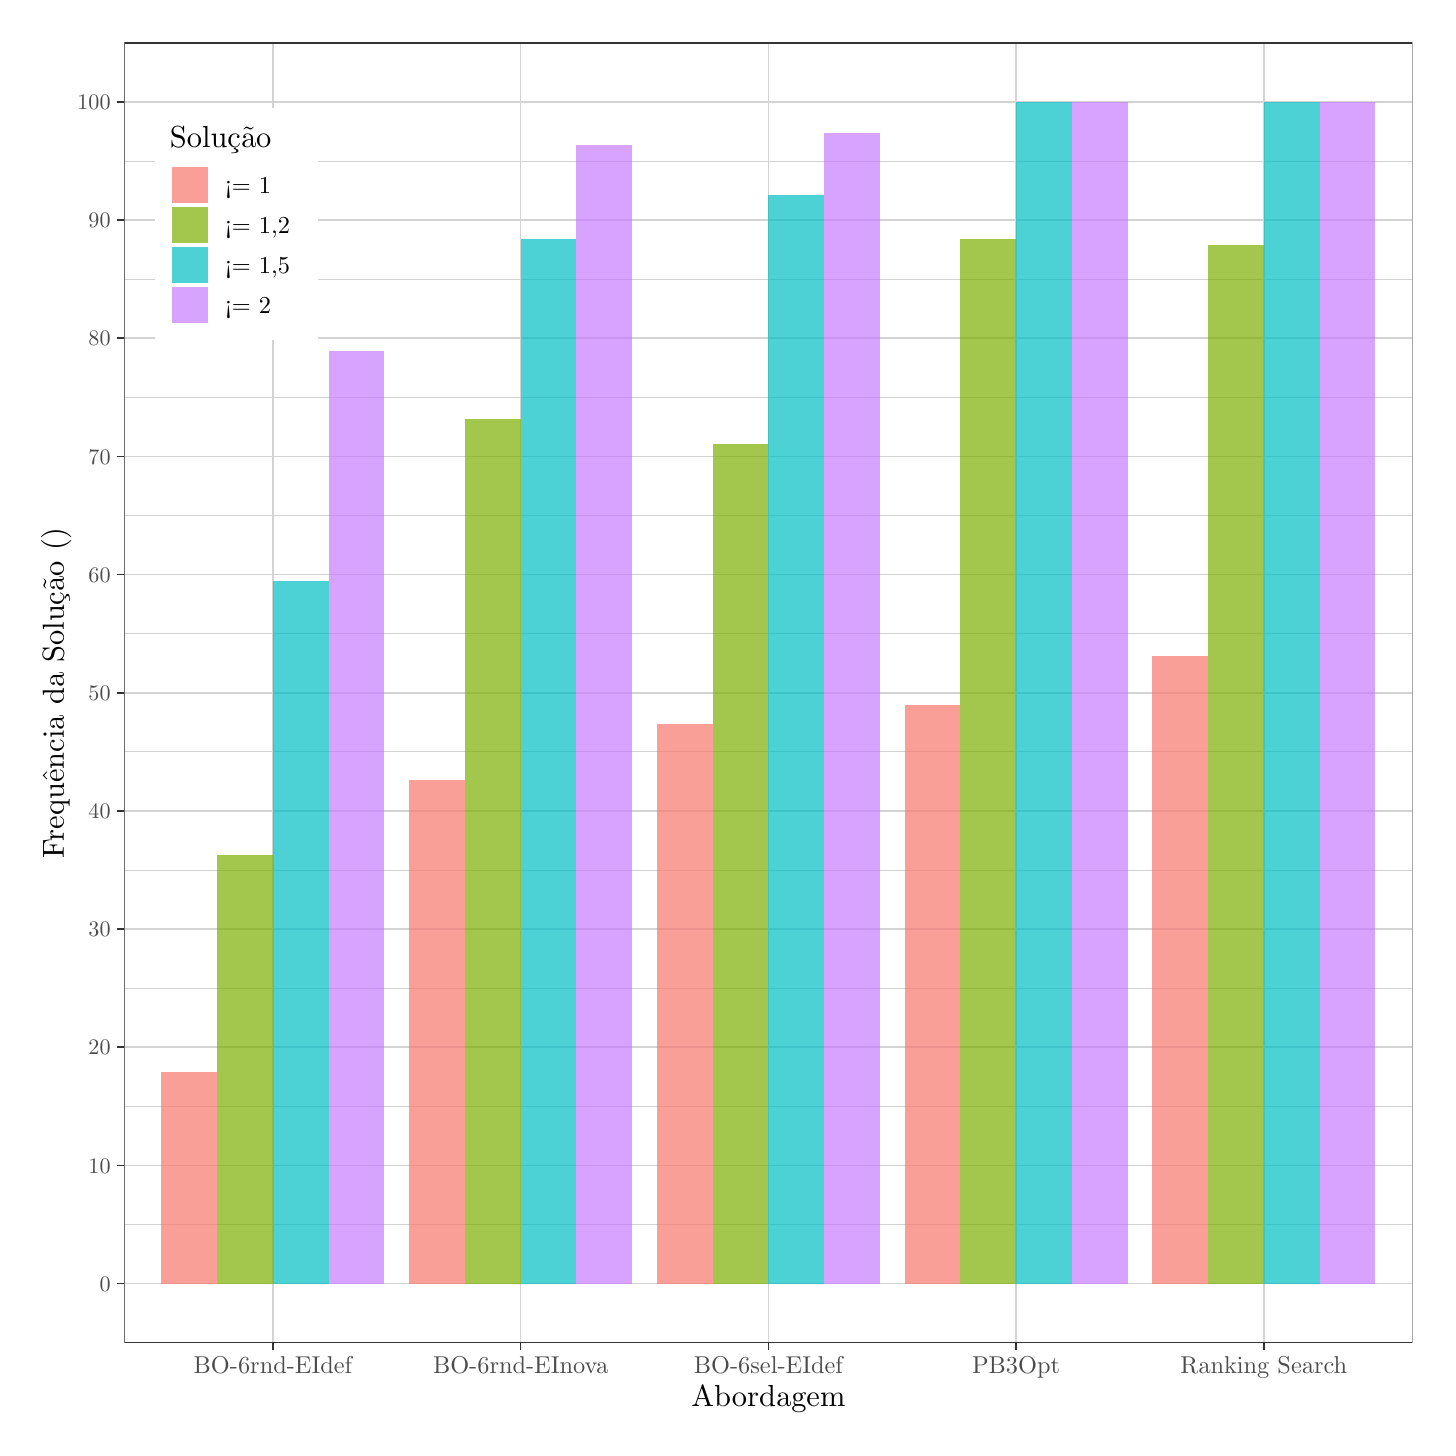
\begin{tikzpicture}[x=1pt,y=1pt]
\definecolor{fillColor}{RGB}{255,255,255}
\path[use as bounding box,fill=fillColor,fill opacity=0.00] (0,0) rectangle (505.89,505.89);
\begin{scope}
\path[clip] (  0.00,  0.00) rectangle (505.89,505.89);
\definecolor{drawColor}{RGB}{255,255,255}
\definecolor{fillColor}{RGB}{255,255,255}

\path[draw=drawColor,line width= 0.6pt,line join=round,line cap=round,fill=fillColor] (  0.00,  0.00) rectangle (505.89,505.89);
\end{scope}
\begin{scope}
\path[clip] ( 34.91, 30.69) rectangle (500.39,500.39);
\definecolor{drawColor}{RGB}{190,190,190}
\definecolor{fillColor}{RGB}{255,255,255}

\path[draw=drawColor,line width= 0.6pt,line join=round,line cap=round,fill=fillColor] ( 34.91, 30.69) rectangle (500.39,500.39);
\definecolor{drawColor}{RGB}{211,211,211}

\path[draw=drawColor,line width= 0.3pt,line join=round] ( 34.91, 30.69) --
	(500.39, 30.69);

\path[draw=drawColor,line width= 0.3pt,line join=round] ( 34.91, 73.39) --
	(500.39, 73.39);

\path[draw=drawColor,line width= 0.3pt,line join=round] ( 34.91,116.09) --
	(500.39,116.09);

\path[draw=drawColor,line width= 0.3pt,line join=round] ( 34.91,158.79) --
	(500.39,158.79);

\path[draw=drawColor,line width= 0.3pt,line join=round] ( 34.91,201.49) --
	(500.39,201.49);

\path[draw=drawColor,line width= 0.3pt,line join=round] ( 34.91,244.19) --
	(500.39,244.19);

\path[draw=drawColor,line width= 0.3pt,line join=round] ( 34.91,286.89) --
	(500.39,286.89);

\path[draw=drawColor,line width= 0.3pt,line join=round] ( 34.91,329.59) --
	(500.39,329.59);

\path[draw=drawColor,line width= 0.3pt,line join=round] ( 34.91,372.29) --
	(500.39,372.29);

\path[draw=drawColor,line width= 0.3pt,line join=round] ( 34.91,414.99) --
	(500.39,414.99);

\path[draw=drawColor,line width= 0.3pt,line join=round] ( 34.91,457.69) --
	(500.39,457.69);

\path[draw=drawColor,line width= 0.3pt,line join=round] ( 34.91,500.39) --
	(500.39,500.39);

\path[draw=drawColor,line width= 0.6pt,line join=round] ( 34.91, 52.04) --
	(500.39, 52.04);

\path[draw=drawColor,line width= 0.6pt,line join=round] ( 34.91, 94.74) --
	(500.39, 94.74);

\path[draw=drawColor,line width= 0.6pt,line join=round] ( 34.91,137.44) --
	(500.39,137.44);

\path[draw=drawColor,line width= 0.6pt,line join=round] ( 34.91,180.14) --
	(500.39,180.14);

\path[draw=drawColor,line width= 0.6pt,line join=round] ( 34.91,222.84) --
	(500.39,222.84);

\path[draw=drawColor,line width= 0.6pt,line join=round] ( 34.91,265.54) --
	(500.39,265.54);

\path[draw=drawColor,line width= 0.6pt,line join=round] ( 34.91,308.24) --
	(500.39,308.24);

\path[draw=drawColor,line width= 0.6pt,line join=round] ( 34.91,350.94) --
	(500.39,350.94);

\path[draw=drawColor,line width= 0.6pt,line join=round] ( 34.91,393.64) --
	(500.39,393.64);

\path[draw=drawColor,line width= 0.6pt,line join=round] ( 34.91,436.34) --
	(500.39,436.34);

\path[draw=drawColor,line width= 0.6pt,line join=round] ( 34.91,479.04) --
	(500.39,479.04);

\path[draw=drawColor,line width= 0.6pt,line join=round] ( 88.62, 30.69) --
	( 88.62,500.39);

\path[draw=drawColor,line width= 0.6pt,line join=round] (178.14, 30.69) --
	(178.14,500.39);

\path[draw=drawColor,line width= 0.6pt,line join=round] (267.65, 30.69) --
	(267.65,500.39);

\path[draw=drawColor,line width= 0.6pt,line join=round] (357.17, 30.69) --
	(357.17,500.39);

\path[draw=drawColor,line width= 0.6pt,line join=round] (446.68, 30.69) --
	(446.68,500.39);
\definecolor{fillColor}{RGB}{248,118,109}

\path[fill=fillColor,fill opacity=0.70] ( 48.34, 52.04) rectangle ( 68.48,128.45);

\path[fill=fillColor,fill opacity=0.70] (137.85, 52.04) rectangle (157.99,234.07);

\path[fill=fillColor,fill opacity=0.70] (227.37, 52.04) rectangle (247.51,254.30);

\path[fill=fillColor,fill opacity=0.70] (316.88, 52.04) rectangle (337.02,261.04);

\path[fill=fillColor,fill opacity=0.70] (406.40, 52.04) rectangle (426.54,279.02);
\definecolor{fillColor}{RGB}{124,174,0}

\path[fill=fillColor,fill opacity=0.70] ( 68.48, 52.04) rectangle ( 88.62,207.11);

\path[fill=fillColor,fill opacity=0.70] (157.99, 52.04) rectangle (178.14,364.42);

\path[fill=fillColor,fill opacity=0.70] (247.51, 52.04) rectangle (267.65,355.43);

\path[fill=fillColor,fill opacity=0.70] (337.02, 52.04) rectangle (357.17,429.60);

\path[fill=fillColor,fill opacity=0.70] (426.54, 52.04) rectangle (446.68,427.35);
\definecolor{fillColor}{RGB}{0,191,196}

\path[fill=fillColor,fill opacity=0.70] ( 88.62, 52.04) rectangle (108.76,305.99);

\path[fill=fillColor,fill opacity=0.70] (178.14, 52.04) rectangle (198.28,429.60);

\path[fill=fillColor,fill opacity=0.70] (267.65, 52.04) rectangle (287.79,445.33);

\path[fill=fillColor,fill opacity=0.70] (357.17, 52.04) rectangle (377.31,479.04);

\path[fill=fillColor,fill opacity=0.70] (446.68, 52.04) rectangle (466.82,479.04);
\definecolor{fillColor}{RGB}{199,124,255}

\path[fill=fillColor,fill opacity=0.70] (108.76, 52.04) rectangle (128.90,389.14);

\path[fill=fillColor,fill opacity=0.70] (198.28, 52.04) rectangle (218.42,463.31);

\path[fill=fillColor,fill opacity=0.70] (287.79, 52.04) rectangle (307.93,467.80);

\path[fill=fillColor,fill opacity=0.70] (377.31, 52.04) rectangle (397.45,479.04);

\path[fill=fillColor,fill opacity=0.70] (466.82, 52.04) rectangle (486.96,479.04);
\definecolor{drawColor}{gray}{0.20}

\path[draw=drawColor,line width= 0.6pt,line join=round,line cap=round] ( 34.91, 30.69) rectangle (500.39,500.39);
\end{scope}
\begin{scope}
\path[clip] (  0.00,  0.00) rectangle (505.89,505.89);
\definecolor{drawColor}{gray}{0.30}

\node[text=drawColor,anchor=base east,inner sep=0pt, outer sep=0pt, scale=  0.80] at ( 29.96, 49.28) {0};

\node[text=drawColor,anchor=base east,inner sep=0pt, outer sep=0pt, scale=  0.80] at ( 29.96, 91.98) {10};

\node[text=drawColor,anchor=base east,inner sep=0pt, outer sep=0pt, scale=  0.80] at ( 29.96,134.68) {20};

\node[text=drawColor,anchor=base east,inner sep=0pt, outer sep=0pt, scale=  0.80] at ( 29.96,177.38) {30};

\node[text=drawColor,anchor=base east,inner sep=0pt, outer sep=0pt, scale=  0.80] at ( 29.96,220.08) {40};

\node[text=drawColor,anchor=base east,inner sep=0pt, outer sep=0pt, scale=  0.80] at ( 29.96,262.78) {50};

\node[text=drawColor,anchor=base east,inner sep=0pt, outer sep=0pt, scale=  0.80] at ( 29.96,305.48) {60};

\node[text=drawColor,anchor=base east,inner sep=0pt, outer sep=0pt, scale=  0.80] at ( 29.96,348.18) {70};

\node[text=drawColor,anchor=base east,inner sep=0pt, outer sep=0pt, scale=  0.80] at ( 29.96,390.88) {80};

\node[text=drawColor,anchor=base east,inner sep=0pt, outer sep=0pt, scale=  0.80] at ( 29.96,433.58) {90};

\node[text=drawColor,anchor=base east,inner sep=0pt, outer sep=0pt, scale=  0.80] at ( 29.96,476.28) {100};
\end{scope}
\begin{scope}
\path[clip] (  0.00,  0.00) rectangle (505.89,505.89);
\definecolor{drawColor}{gray}{0.20}

\path[draw=drawColor,line width= 0.6pt,line join=round] ( 32.16, 52.04) --
	( 34.91, 52.04);

\path[draw=drawColor,line width= 0.6pt,line join=round] ( 32.16, 94.74) --
	( 34.91, 94.74);

\path[draw=drawColor,line width= 0.6pt,line join=round] ( 32.16,137.44) --
	( 34.91,137.44);

\path[draw=drawColor,line width= 0.6pt,line join=round] ( 32.16,180.14) --
	( 34.91,180.14);

\path[draw=drawColor,line width= 0.6pt,line join=round] ( 32.16,222.84) --
	( 34.91,222.84);

\path[draw=drawColor,line width= 0.6pt,line join=round] ( 32.16,265.54) --
	( 34.91,265.54);

\path[draw=drawColor,line width= 0.6pt,line join=round] ( 32.16,308.24) --
	( 34.91,308.24);

\path[draw=drawColor,line width= 0.6pt,line join=round] ( 32.16,350.94) --
	( 34.91,350.94);

\path[draw=drawColor,line width= 0.6pt,line join=round] ( 32.16,393.64) --
	( 34.91,393.64);

\path[draw=drawColor,line width= 0.6pt,line join=round] ( 32.16,436.34) --
	( 34.91,436.34);

\path[draw=drawColor,line width= 0.6pt,line join=round] ( 32.16,479.04) --
	( 34.91,479.04);
\end{scope}
\begin{scope}
\path[clip] (  0.00,  0.00) rectangle (505.89,505.89);
\definecolor{drawColor}{gray}{0.20}

\path[draw=drawColor,line width= 0.6pt,line join=round] ( 88.62, 27.94) --
	( 88.62, 30.69);

\path[draw=drawColor,line width= 0.6pt,line join=round] (178.14, 27.94) --
	(178.14, 30.69);

\path[draw=drawColor,line width= 0.6pt,line join=round] (267.65, 27.94) --
	(267.65, 30.69);

\path[draw=drawColor,line width= 0.6pt,line join=round] (357.17, 27.94) --
	(357.17, 30.69);

\path[draw=drawColor,line width= 0.6pt,line join=round] (446.68, 27.94) --
	(446.68, 30.69);
\end{scope}
\begin{scope}
\path[clip] (  0.00,  0.00) rectangle (505.89,505.89);
\definecolor{drawColor}{gray}{0.30}

\node[text=drawColor,anchor=base,inner sep=0pt, outer sep=0pt, scale=  0.88] at ( 88.62, 19.68) {BO-6rnd-EIdef};

\node[text=drawColor,anchor=base,inner sep=0pt, outer sep=0pt, scale=  0.88] at (178.14, 19.68) {BO-6rnd-EInova};

\node[text=drawColor,anchor=base,inner sep=0pt, outer sep=0pt, scale=  0.88] at (267.65, 19.68) {BO-6sel-EIdef};

\node[text=drawColor,anchor=base,inner sep=0pt, outer sep=0pt, scale=  0.88] at (357.17, 19.68) {PB3Opt};

\node[text=drawColor,anchor=base,inner sep=0pt, outer sep=0pt, scale=  0.88] at (446.68, 19.68) {Ranking Search};
\end{scope}
\begin{scope}
\path[clip] (  0.00,  0.00) rectangle (505.89,505.89);
\definecolor{drawColor}{RGB}{0,0,0}

\node[text=drawColor,anchor=base,inner sep=0pt, outer sep=0pt, scale=  1.10] at (267.65,  7.64) {Abordagem};
\end{scope}
\begin{scope}
\path[clip] (  0.00,  0.00) rectangle (505.89,505.89);
\definecolor{drawColor}{RGB}{0,0,0}

\node[text=drawColor,rotate= 90.00,anchor=base,inner sep=0pt, outer sep=0pt, scale=  1.10] at ( 13.08,265.54) {Frequência da Solução ()};
\end{scope}
\begin{scope}
\path[clip] (  0.00,  0.00) rectangle (505.89,505.89);
\definecolor{fillColor}{RGB}{255,255,255}

\path[fill=fillColor] ( 45.92,392.87) rectangle (104.73,476.90);
\end{scope}
\begin{scope}
\path[clip] (  0.00,  0.00) rectangle (505.89,505.89);
\definecolor{drawColor}{RGB}{0,0,0}

\node[text=drawColor,anchor=base west,inner sep=0pt, outer sep=0pt, scale=  1.10] at ( 51.42,462.76) {Solução};
\end{scope}
\begin{scope}
\path[clip] (  0.00,  0.00) rectangle (505.89,505.89);
\definecolor{fillColor}{RGB}{255,255,255}

\path[fill=fillColor] ( 51.42,441.74) rectangle ( 65.87,456.19);
\end{scope}
\begin{scope}
\path[clip] (  0.00,  0.00) rectangle (505.89,505.89);
\definecolor{fillColor}{RGB}{248,118,109}

\path[fill=fillColor,fill opacity=0.70] ( 52.13,442.45) rectangle ( 65.16,455.48);
\end{scope}
\begin{scope}
\path[clip] (  0.00,  0.00) rectangle (505.89,505.89);
\definecolor{fillColor}{RGB}{255,255,255}

\path[fill=fillColor] ( 51.42,427.28) rectangle ( 65.87,441.74);
\end{scope}
\begin{scope}
\path[clip] (  0.00,  0.00) rectangle (505.89,505.89);
\definecolor{fillColor}{RGB}{124,174,0}

\path[fill=fillColor,fill opacity=0.70] ( 52.13,427.99) rectangle ( 65.16,441.03);
\end{scope}
\begin{scope}
\path[clip] (  0.00,  0.00) rectangle (505.89,505.89);
\definecolor{fillColor}{RGB}{255,255,255}

\path[fill=fillColor] ( 51.42,412.83) rectangle ( 65.87,427.28);
\end{scope}
\begin{scope}
\path[clip] (  0.00,  0.00) rectangle (505.89,505.89);
\definecolor{fillColor}{RGB}{0,191,196}

\path[fill=fillColor,fill opacity=0.70] ( 52.13,413.54) rectangle ( 65.16,426.57);
\end{scope}
\begin{scope}
\path[clip] (  0.00,  0.00) rectangle (505.89,505.89);
\definecolor{fillColor}{RGB}{255,255,255}

\path[fill=fillColor] ( 51.42,398.37) rectangle ( 65.87,412.83);
\end{scope}
\begin{scope}
\path[clip] (  0.00,  0.00) rectangle (505.89,505.89);
\definecolor{fillColor}{RGB}{199,124,255}

\path[fill=fillColor,fill opacity=0.70] ( 52.13,399.09) rectangle ( 65.16,412.12);
\end{scope}
\begin{scope}
\path[clip] (  0.00,  0.00) rectangle (505.89,505.89);
\definecolor{drawColor}{RGB}{0,0,0}

\node[text=drawColor,anchor=base west,inner sep=0pt, outer sep=0pt, scale=  0.88] at ( 71.37,445.93) {<= 1};
\end{scope}
\begin{scope}
\path[clip] (  0.00,  0.00) rectangle (505.89,505.89);
\definecolor{drawColor}{RGB}{0,0,0}

\node[text=drawColor,anchor=base west,inner sep=0pt, outer sep=0pt, scale=  0.88] at ( 71.37,431.48) {<= 1,2};
\end{scope}
\begin{scope}
\path[clip] (  0.00,  0.00) rectangle (505.89,505.89);
\definecolor{drawColor}{RGB}{0,0,0}

\node[text=drawColor,anchor=base west,inner sep=0pt, outer sep=0pt, scale=  0.88] at ( 71.37,417.03) {<= 1,5};
\end{scope}
\begin{scope}
\path[clip] (  0.00,  0.00) rectangle (505.89,505.89);
\definecolor{drawColor}{RGB}{0,0,0}

\node[text=drawColor,anchor=base west,inner sep=0pt, outer sep=0pt, scale=  0.88] at ( 71.37,402.57) {<= 2};
\end{scope}
\end{tikzpicture}
